\chapter{Literature Review}
\label{Chapter2}

% 转折
% \subsubsection{Approximate Bayesian Inference Intuition}
\section{Bayesian Inference Paradigm}
\label{bayeisanP}
\textbf{Why Bayesian}
Bayesian inference approaches offer numerous advantages in the statistical community and application areas, especially in situations where data is scarce. In cases where effective data is extremely rare and insufficient, an appropriate prior choice can provide significant benefits, particularly in medical problems. Unlike frequentist inference approaches that treat parameter estimates as fixed values, Bayesian inference approaches regard parameter estimates as random variables that have probability distributions. This unique feature allows for interval estimates and error variances to be generated, providing a more comprehensive understanding of uncertainty and increasing confidence in interpreting parameter estimates. By incorporating prior knowledge and probability distributions, Bayesian Inference approaches offer a more flexible and intuitive framework for statistical analysis.

\textbf{Bayesian Inference Intuition}
The Bayesian inference approach stems from the Bayes rule, which is defined as Equation (\ref{eq:Bayesrule}) based on theory developed by \cite{Beech1959}. Suppose $\theta$ is our model parameter of interest, $\mathcal{D}$ is data, then $p(\theta)$ is known as a prior distribution, which offers pre-existing knowledge or information about $\theta$. Posterior distribution $p(\theta|\mathcal{D})$ refers to the likelihood conditioning on the data $\mathcal{D}$.
Incorporating information from current data and prior knowledge, posterior distribution can be then inferred and simplified to Equation (\ref{eq:simBayesrule}), as the value of $p(\mathcal{D})$ is constant and insignificant for determining the overall posterior distribution. 
\begin{equation}
	p(\theta|\mathcal{D}) = \frac{p(\mathcal{D}|\theta)p(\theta)}{p(\mathcal{D})},
	\label{eq:Bayesrule}
\end{equation}
\begin{equation}
	p(\theta|\mathcal{D}) \propto p(\mathcal{D}|\theta)p(\theta),
	\label{eq:simBayesrule}
\end{equation}
\section{Least Absolute Shrinkage and Selection Operator (LASSO) penalized regression}
\subsection{Lasso penalty formulation}
The constraint form of lasso can be shown by Equation \ref{eq:lasso2}, where $t \geq 0$ is denoted as a tuning term, the regression coefficient is $\beta$, $||\beta||_1$ is the $l_1$ norm of beta, $||y-X\beta||_2$ is the $l_2$ norm: of residual value, the data matrix is $X$, the response variable is $y$. The estimation for lasso estimate $\hat{\beta}_{lasso}$ is defined by \autoref{eq:lasso2}. 

\begin{equation}
	\label{eq:lasso2}
	\hat{\beta}_{lasso} = \underset{\beta}{\operatorname{argmin}} ||y-X\beta||_2, s.t. ||\beta||_1 \leq t, t \geq 0.
\end{equation}
In order to transform the constraint form of the lasso to penalty form, the Lagranage multiplier method, as a pivotal technique for transforming a constraint optimization system into an unconstrained penalty formulation of the system has been used. The Lagrangian function for constrained Lasso Regression is constructed by \autoref{eq:lagrangelasso}
\begin{equation}
	\label{eq:lagrangelasso}
	\mathcal{L}(\beta,\lambda) =  ||y-X\beta||_2 + \lambda||\beta||_1 - \lambda t, \lambda \geq 0
\end{equation}
Since the objective function contains a quadratic term $||y-X\beta||_2$ with a linear term $\lambda||\beta||_1 - \lambda t)$, leading to a convex optimization problem. Due to the strong duality theorem in convex optimization system, therefore the penalty formulation of lasso regression can be deduced as Equation \autoref{eq:lasso1}, is equivalent to constraint form \autoref{eq:lasso2} after ignoring the unaffected constant $-\lambda t$.


Graphical demonstration of the lasso for Equation \ref{eq:lasso2} and Equation \ref{eq:lasso1} can also be found on the left-hand side of Figure \ref{fig:lassodemo}, where the squared constraint set is drawn, in addition to the contour line of the regression coefficient. The penalty term $\lambda$ controls the strength of the penalization in Lasso regression. When the value of $\lambda$ is set higher, a more sparse solution is facilitated. This forces the estimated coefficients to lie closer to the axis of each parameter, as shown in \ref{fig:lassodemo}. As a result, Lasso regression coefficients are more likely to intersect with the corners of the squared constraint set, leading to the occurrence of sparse estimated regression coefficients. By encouraging sparsity, Lasso regression provides a useful tool for variable selection and reducing model complexity, leading to more interpretable and generalizable models. On the other hand, ridge regression uses a $l_2$ penalty to estimate the regression coefficients, but it tends to gain a non-sparse solution due to the circled constraint set for $\beta$.

\begin{figure}
	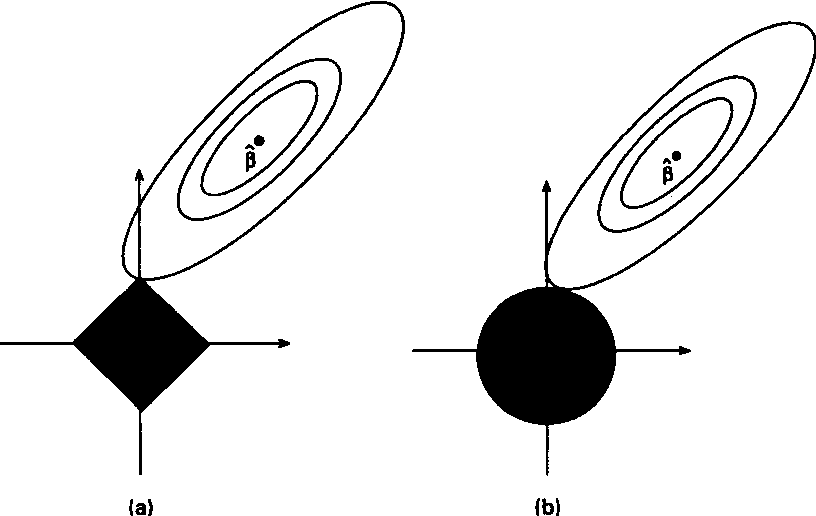
\includegraphics[width=\linewidth]{lassodemo}
	\caption{Graphical comparison between lasso regression and ridge regression}
	\label{fig:lassodemo}
\end{figure}

\section{Bayesian Lasso}
\subsection{Bayesian Lasso model}
\cite{park_casella_2008} proposed an alternative formula for the conditional Laplace prior, which takes the form of \autoref{eq:LassoPrior} and is expanded in \autoref{eq:expandLasso}. This approach offers a Bayesian interpretation of the Lasso penalty and provides a framework for incorporating prior information into the variable selection process. By using the conditional Laplace prior, the Bayesian Lasso regression model can be tuned to strike a balance between sparsity and estimation accuracy, resulting in a more robust and interpretable model.
\begin{equation}
	\label{eq:expandLasso}
	\pi(\beta) = \prod_{j=1}^p \frac{\lambda}{2} e^{-\lambda|\beta_j|}
\end{equation}

For a given variance, the mode of posterior form in \autoref{eq:fullCondLasso} is consistent with the estimate of the lasso equation in \autoref{eq:lasso1}, but it will hinder the Bayesian interpretation, inference, and variable selection since the bayesian predictive distribution makes future inference via a posterior mean instead of posterior mode.
In addition, if a variance is unknown, the posterior will be a multimodal distribution, the derivation has been provided by the appendix from \cite{park_casella_2008}.
\begin{equation}
	\label{eq:fullCondLasso}
	\pi(\beta,\sigma^2|\tilde{y}) \propto \pi(\sigma^2)(\sigma^2)^{-(n-1)/2}\textnormal{exp}\left(\frac{1}{2\sigma^2}(\tilde{y}-X\beta)^T(\tilde{y}-X\beta)-\lambda\sum_{j=1}^p|\beta_j|\right)
\end{equation}
\begin{equation}
	\label{eq:lassocondprior}
	\pi(\beta |\sigma^2) = \prod_{j=1}^p \frac{\lambda}{2\sqrt{\sigma^2}} e^{-\lambda|\beta_j|/\sqrt{\sigma^2}}
\end{equation}
To remedy this issue, a conditional Laplacian prior from \ref{eq:lassocondprior} with respect to Equation(\ref{eq:expandLasso}) has been designed, ensuring the unimodality of the posterior for $\beta$, and the current prior with respect to $\beta$, $\sigma^2$  can be written as
\begin{equation}
	\label{eq:lassoprior}
	\pi(\beta,\sigma^2) \propto \pi(\sigma^2) \prod_{j=1}^p \frac{\lambda}{2\sqrt{\sigma^2}} e^{-\lambda|\beta_j|/\sqrt{\sigma^2}},
\end{equation}
which can result in the unimodal joint posterior distribution $\pi(\beta,\sigma^2|\tilde{y})$ of $\beta$ and $\sigma^2 > 0$ under the new prior \ref{eq:lassoprior}, given an improper prior selection for $\pi(\sigma^2) = \frac{1}{\sigma^2}$ and $\lambda \geq 0$.
Additionally, an additional latent variable $\tau$ is introduced as a scale mixture of Gaussians for reformulation of conditional prior \ref{eq:lassocondprior} as \ref{eq:MofN}, which can be regarded as corresponding weight assigned to each regression coefficient. If $\tau_j$ goes to 0 then the corresponding regression coefficient will be shrunk towards zero accordingly.
\begin{equation}
	\label{eq:MofN}
	\frac{\alpha}{2}e^{-\alpha|z|} = \int_{0}^{\infty} \frac{1}{\sqrt{2\pi s}}e^{-z^2/(2s)} \frac{\alpha^2}{2}e^{-\alpha^2s/2}ds, \alpha > 0
\end{equation}

Finally, the hierarchical Bayesian Lasso model functional form can be written as Equation (\ref{eq:blassocond}).
\begin{equation}
	\label{eq:blassocond}
	\begin{multlined}
		y|\mu,X,\beta,\sigma^2 \sim N_n(\mu + X\beta,\sigma^2I)\\
		\beta|\tau_1^2,...,\tau_p^2 \sim N_p(0,\sigma^2D_{\tau})\\
		D_{\tau} = diag(\tau_1^2,...,\tau_p^2)\\
		\tau_1^2..,\tau_p^2 \sim \prod_{j=1}^p \frac{\lambda^2}{2} e^{-\lambda^2\tau_j^2/2}d\tau_j^2, \tau_1^2,..,\tau_j^2 > 0\\
		\sigma^2 \sim \pi(\sigma^2) = 1/\sigma^2, \sigma^2 > 0\\.
	\end{multlined}
\end{equation}

\subsection{Bayesian Lasso Gibbs Sampler}
\subsubsection{Gibbs Sampler}
\cite{4767596} introduced a special case of the Metropolis-Hastings algorithm called the Gibbs sampler. As a Markov Chain Monte Carlo sampling algorithm, it can be used for efficient sampling of any probability density function, given the posterior form from the corresponding conditional distribution. In each iteration, each parameter of interest is sampled once by conditional distribution for the current iteration. After running the chain for long enough iterations, it returns posterior distribution samples with descent approximation accuracy after discarding samples in the burn-in period. Notice that, the functional form of conditional distribution given any other parameter of interest has to be acquired. In this study, we need to have the marginal distributions of  $(\beta,\sigma^2,\tau)$:
$$
\begin{multlined}
	p(\mathbf{\beta}|\mathcal{D},\sigma^2,\mathbf{\tau}^2)\\
	p(\mathbf{\sigma}^2|\mathcal{D},\beta,\mathbf{\tau}^2)\\
	p(\tau|\mathcal{D},\beta,\sigma^2)\\
\end{multlined}
$$
After getting the functional form and ignoring the normalizing constant, we can infer the category of the probability distribution for each expression, and we can sample from the corresponding distribution.

\textbf{Initial Setting}:
In the initial setting we consider that: $\lambda$ is fixed, and $\sigma^2$ has a a Gamma distribution with parameter $a$ and $b$: $\pi(\sigma^2) = \frac{b^a}{\Gamma(a)} (\sigma^2)^{-a-1}e^{-b^2/\sigma^2},\sigma^2>0,a>0,b>0$ \\
Our first step is to write the joint distribution: $p(\mathbf{\beta},\mathbf{\tau}^2,\sigma^{2},\mathcal{D})$

\textbf{Joint distributional form}:
Given \autoref{eq:blassocond}, we can write the joint distribution as
\begin{equation}
	\begin{multlined}
		p(\tilde{y},\beta,\tau^2,\sigma^2) = p(\tilde{y}|\beta,\sigma^2,\tau)p(\sigma^2)\prod_{j=1}^p p(\beta|\sigma^2,\tau_j)p(\tau_j^2)\\
		=\frac{1}{(2\pi\sigma^2)^{\frac{n}{2}}} e^{\frac{-(\tilde{y} -X\beta)^T(\tilde{y}-X\beta)}{2\sigma^2}}
		\frac{b^a}{\Gamma(a)} (\sigma^2)^{-a-1}e^{-b^2/\sigma^2}
		\prod_{j=1}^p \frac{1}{(2\sigma^2\tau_j^2)^{1/2}}e^{-\frac{-1}{2\sigma^2\tau_j^2}\beta_j^2}\frac{\lambda^2}{2}e^{-\lambda^2\tau_j^2/2}
	\end{multlined}
\end{equation}

\textbf{Full conditional distribution of $\beta$}:

\begin{equation}
	\begin{multlined}
		p(\beta | \tilde{y},\tau,\sigma^2) \propto  	p(\tilde{y},\beta,\tau,\sigma^2)
	\end{multlined}
\end{equation}
Recognizing the term without $\beta$ as constant, the conditional distribution of $\beta$ can be simplified to
\begin{equation}
	\begin{multlined}
		p(\beta|\tilde{y},\sigma^2,\tau^2) \propto \textnormal{exp}(\frac{\beta^TX^TX\beta - 2y^TX\beta +\lambda^2\beta^TA^{-1}\beta}{-2\sigma^2}), A = diag(\tau)\\
		=  \textnormal{exp}(-\frac{1}{2}\beta^T(\frac{X^TX + \lambda^2A^{-1}}{-2\sigma^2})\beta + \frac{\tilde{y}^TX\beta}{\sigma^2})\\
		\sim \textnormal{MVN}(\mu^*,\Sigma^*)\\
		\textnormal{where } \mu^* = (X^TX+\lambda^2A^{-1})^{-1}X^Ty, \Sigma^* = (X^TX+\lambda^2A^{-1})^{-1}\sigma^2\\
	\end{multlined}
\end{equation}
So we can sample $\beta$ from a multivariate normal distribution with its corresponding mean and variance.

\textbf{Full conditional distribution of $\sigma^2$}:

\begin{equation}
	\begin{multlined}
		p(\sigma^2|\tilde{y},\beta,\tau^2) \propto  	p(\tilde{y},\beta,\tau^2,\sigma^2)  \\
		= (\sigma^2)^{-\frac{n}{2}-\frac{p}{2}-a-1}\textnormal{exp}(-\frac{1}{2\sigma^2}(\tilde{y}-X\beta)^T(\tilde{y}-X\beta)+\frac{1}{2\sigma^2}\beta^TD_{\tau}\beta+\frac{b}{\sigma^2}).\\
		\sim \textnormal{Inverse-Gamma}(\alpha^*,\beta^*)\\
		\textnormal{where } \alpha^* = \frac{n}{2}+\frac{p}{2}+a, \beta^* = 
		(\tilde{y}-X\beta)^T(\tilde{y}-X\beta)/2 + \beta^TD_{\tau}\beta/2 +b
	\end{multlined}
\end{equation}

\textbf{Full conditional distribution of $\tau_j^2$}:
\begin{equation}
	\begin{multlined}
		p(\tau_j^2|\tilde{y},\beta,\sigma^2) \propto  	p(\tilde{y},\beta,\tau^2,\sigma^2)  
		= \frac{1}{\sqrt{\frac{2\pi\sigma^2\tau_j}{\lambda^2}}}\textnormal{exp}(-\frac{-\beta_j^2\lambda^2}{2\sigma^2\tau_j})\textnormal{exp}(-\frac{1}{2}\tau_j)]\\
		\sim GIG(a^*,b^*,p^*)\\
		\textnormal{where GIG is generalized inverse gaussian distribution with parameters } a^* = 1, b^* = \frac{\beta_j^2\lambda^2}{\sigma^2}, p = \frac{1}{2}
	\end{multlined}
\end{equation}

\textbf{Summary}
The Gibbs sampler can be established by the following algorithm \autoref{alg:algorithm1}.
\begin{algorithm}
	\caption{Gibbs Sampler for the Bayesian Lasso}
	\begin{algorithmic}[1]
		
		\State Given $\lambda^2>0, \mathbf{\tau}^{(1)} = \mathbf{1_n}, \sigma^{2(1)} =1 , t=1$ \Comment{Initial Setting}
		\While{$t \leq 10^5$}
		
		\State Sampling $\mathbf{\beta}^{(t+1)} \sim \textnormal{MVN}((X^TX+\lambda^2A^{-1})^{-1}X^Ty,(X^TX+\lambda^2A^{-1})^{-1}\sigma^2) $  \Comment{Generate sample $\beta$}
		\State Sampling $\sigma^{2(t+1)} \sim IG(\frac{n}{2}+\frac{p}{2}+a,\frac{||y-X\beta||_2^2}{2}+\frac{\lambda^2\sum_j{\beta_j^2}}{2\tau_j}+b)$ \Comment{Generate sample $\sigma^2$}
		\For{$j$=1,...,$p$}
		\State Sampling $\mathbf{\tau}_j^{2(t+1)} \sim GIG(1,\frac{\beta_j^2\lambda^2}{\sigma^2},1/2)$ \Comment{Generate sample $\tau_j$}
		\EndFor
		\State $t \leftarrow t + 1$
		\EndWhile  \label{roy's loop}
		\State return $\beta,\sigma^2,\tau^2$
		
		
	\end{algorithmic}
	\label{alg:algorithm1}
\end{algorithm}

% \section{Bayesian Paradigm}
\textbf{Automatic selection of the penalty parameter $\lambda$:}
A common choice of penalty parameter $\lambda$ in the non-bayesian paradigm involves a cross-validation approach, which is time-consuming and computationally challenging, especially for large datasets.
\cite{park_casella_2008} set a hyperprior to $\lambda^2$ as \ref{eq:hyperprior}, instaed of $\lambda$ to facilitate conjugacy.
According to \cite{park_casella_2008}, there is some additional notification of choosing prior, which involves: firstly, to avoid mixing issue, the prior distribution for $\lambda^2$ should reach zero asymptotically with a descent speed as $\lambda^2 $ goes to infinity, Secondly, the density at maximum likelihood estimate should be assigned with enough probability density with an overall flat distribution.
\begin{equation}
	\label{eq:hyperprior}
	\pi(\lambda^2) = \frac{\delta^\gamma}{\Gamma(\gamma)}(\lambda^2)^{\gamma-1}e^{-\delta\lambda^2}, \textnormal{for } \delta>0, \gamma>0, \lambda^2>0
\end{equation}

The penalty parameter is the extent of penalization of the non-zero coefficient, which is also a compromise between model simplicity and fitting capability to data in the frequentist lasso setting. According to the posterior form of $\tau_j$, $\lambda$ controls the shape of the generalized inverse-Gaussian posterior distribution of $\tau_j$ as shown before.

To obtain the posterior form of $\lambda$, we need to incorpoate a proper hyperprior distribution to the joint distribution $p(y,\beta,\sigma^2,\tau)$. First, assuming the prior of $\lambda^2$ is with shape and rate parameters $\theta$ and $\gamma$, respectively.
\begin{equation}
	\label{eq:hyperpriorGamma}
	\begin{multlined}
		p(\lambda^2|\tilde{y},\beta,\sigma^2,\tau^2) \propto  	p(\tilde{y},\beta,\tau^2,\sigma^2,\lambda)  \\
		= (\prod_{j=1}^p \frac{\lambda^2}{2} e^{-\lambda^2\tau_j^2/2})(\lambda^2)^{\gamma-1}e^{-\delta\lambda^2}\\
		= (\lambda^2)^{p+\gamma-1}e^{-\lambda^2(\frac{1}{2}\sum_{j=1}^p \tau_j^2+\delta)}
	\end{multlined}
\end{equation} 
Thus, the posterior distribution of $\lambda^2$ is still following a Gamma distribution, with a shape parameter $p+\gamma-1$ and rate parameter $\sum_{j=1}^p \tau_j^2+\delta$. The $\lambda^2$ can be sampled by \ref{eq:hyperpriorGamma}, based on using an augmented Gibbs sampler.

\section{Expectation Maximization}
Even though the posterior distribution can be sampled by the Gibbs sampler in the last subsection, the sparsity nature of the Bayesian lasso is not captured by the posterior mean given by Gibbs Sampler. The posterior mode calculated by Bayesian Expectation Maximization, however, could capture the posterior mode and preserve the sparsity feature of the basic lasso.

\subsection{Classical Expectation Maximization}
The expectation maximization (EM) algorithm was proposed by \cite{EM}. It is an iterative approach for seeking the maximum likelihood estimate of parameters for probabilistic models that have missing data or latent variables.
The application of the EM algorithm includes the inference of the parameters of the Gaussian Mixture model etc. The EM algorithm involves two main steps, which are E-steps and M-steps.
Suppose $Z$ is the set of latent variables, $X$ is the set of the entire set of observed variables, and $\theta$ is a target parameter. $t$ refers to the step during iteration, $\textnormal{log}(P(X, Z|\theta)))$ refers to the complete log-likelihood of data, and $\textnormal{log}(P(X|\theta)))$ refers to the incomplete log-likelihood of data without considering the hidden variables.
\subsubsection{E-steps}
By calculating the posterior distribution of the hidden variable given by the observed data and current parameter estimates, the purpose of this step is to compute the expectation of the latent variables by observed data, which is equivalent to calculating the expected value of the complete log-likelihood given the current parameter estimation and observed data.
Mathematically, the E-step involves calculating the expectation of the complete data log-likelihood with respect to the conditional distribution of the hidden data given the observed data and current parameter estimates:
\begin{equation}
	Q(\theta,\theta^{(t-1)}) = E_{Z|X,\theta^{(t-1)}}[\textnormal{log}(P(X,Z|\theta))].
\end{equation}
Overall, the purpose of this step is to use the observed data to estimate and update the values of the missing data

\subsubsection{M-steps}
The purpose of this step is to update the parameters that could maximize the expected complete data log-likelihood generated by the E-step, according to the current estimates
\begin{equation}
	\theta^{(t)} = 
	\operatorname*{argmax}_{\theta} Q(\theta,\theta^{(t-1)}).
\end{equation}
The algorithm runs until the difference between $\theta^{(t)}$ and $\theta^{(t-1)}$ is within an acceptable tolerance. 
The advantages and disadvantages of the EM algorithm are as follows: EM algorithm guarantees the increase of likelihood for each iteration according to \cite{EM}, which enables the EM algorithm to become a greedy algorithm. However, it might suffer from slow convergence speed, sensitivity to the initial parameter value, and convergence to a local optimum if there are multiple local optima in the optimization error surface.


\subsection{Bayesian Expectation Maximization}
The Bayesian EM algorithm incorporates the idea of EM algorithm and Bayesian inference for the estimation of the probabilistic model when the data has missing or hidden values. As opposed to the traditional EM approach, the Bayesian EM approach incorporates prior knowledge of the parameter, for the estimation of the posterior mode $p(\theta|\mathcal{D})$, considering the prior distribution as $p(\theta)$, the Bayes rule can be written in the log scale
\begin{equation}
	\label{eq:logbayesrule}
	\textnormal{ln} p(\theta|\mathcal{D}) = \textnormal{ln}(p(\mathcal{D}|\theta)) + \textnormal{ln}(p(\theta)) - \textnormal{ln}(p(\mathcal{D}))
\end{equation}
We can then further expand \autoref{eq:logbayesrule} to \autoref{eq:expansionBR}
\begin{equation}
	\label{eq:expansionBR}
	\textnormal{ln} p(\theta|\mathcal{D}) = Q(\theta,\theta^{(old)}) + \textnormal{KL}(q||p(Z|X)) + \textnormal{ln}(p(\theta)) - \textnormal{ln}(p(\mathcal{D}))
\end{equation}
, where KL$(P||Q)$ is defined by \autoref{eq:KL2}

\subsection{Bayesian EM for Bayesian Lasso model}
In order to deploy the Bayesian EM algorithm to the Bayesian Lasso model for attaining the posterior mode, our purpose is to iteratively calculate 
\begin{equation}
	\theta_1^{(t+1)} = \operatorname*{argmax}_{\theta_1} [E_{\theta_2|\tilde{y},\theta_1^{(t)}}[\textnormal{log}p(y,\theta_1,\theta_2)]].
\end{equation}

\subsubsection{E-step}
Using the same notation as before, firstly, the complete log-likelihood can be written as \autoref{eq:CompleteLL}
\begin{equation}
	\label{eq:CompleteLL}
	\textnormal{log}(p(\theta_1,\theta_2,\tilde{y})) \propto -\frac{n+p}{2}\textnormal{log}(\sigma^2) - \frac{||\tilde{y}-X\beta||_2^2}{2\sigma^2} - \frac{1}{2\sigma^2}\beta^TE_{\theta_2|\tilde{y},\theta_1^{(t)}}[D_{\tau}]\beta - \frac{b}{\sigma^2}
\end{equation}
given $\theta_1 = (\beta,\sigma^2)$ as a set of observed variables, $\theta_2 = \tau^2 = (\tau_1^2,..,\tau_j^2)$ as a set of latent variables, y is response variable.


\begin{equation}
	\label{eq:nextloglL}
	E_{\theta_2|\tilde{y},\theta_1^{(t)}}[\textnormal{log } p(y,\theta_1,\theta_2)] = -\frac{n}{2} \textnormal{log}(\sigma^{2(t)}) - \frac{||y-X\beta^{(t)}||_2^2}{2\sigma^{2(t)}} - E_{\theta_2 |\tilde{y},\theta_1^{(t)}}\left[\sum_{j=1}^p \frac{\lambda^2\beta_j^2}{2\sigma^2\tau_j^2}\right] -(a+1)\textnormal{log}(\sigma^{2(t)})) - \frac{b}{\sigma^{2(t)}}.
\end{equation}
Next, we need to take the expectation of hidden variables: $E_{\theta_2 |\tilde{y},\theta_1^{(t)}}[\sum_{j=1}^p \frac{\lambda^2\beta_j^2}{2\sigma^2\tau_j^2}]$. After extracting constant with respect to $\theta_2$, required formulation is $E_{\theta_2 |\tilde{y},\theta_1^{(t)}}[\frac{1}{\tau_j}]$. Given the fact that $\tau_j^2|\sigma^2,\tilde{y},\beta \sim GIG(1,\frac{\beta_j^2\lambda^2}{\sigma^2},\frac{1}{2})$ and the special property of Generalized Inverse Gaussian distribution that if $X \sim GIG(a,b,p)$, then $\frac{1}{X} \sim GIG(b, a,-p)$, the distribution of $\frac{1}{\tau_j^2}$ can be rearranged to  $\frac{1}{\tau_j^2}|\sigma^2,\tilde{y},\beta \sim GIG(\frac{\beta_j^2\lambda^2}{\sigma^2},1,-\frac{1}{2})$.
However, taking expectations with respect to Generalized Gaussian Distribution is still complicated and requires advanced mathematical operation and functional properties such as modified Bessel function. Thus, we can continue converting the distribution into an Inverse Gaussian distribution family, which renders $\frac{1}{\tau_j^2}|\sigma^2,\theta_1,\tilde{y} \sim \text{InverseGaussian}(b^{-\frac{1}{2}},1)$. Rewriting \autoref{eq:nextloglL} can lead to the final conditional expectation form can be written as:
\begin{equation}
	Q(\theta,\theta^{(t)}) = -\left(\frac{n}{2}+\frac{p}{2}+a+1\right)\log(\sigma^2)-\frac{b}{\sigma^2}-\frac{||y-X\beta||_2^2}{2\sigma^2}-\frac{\lambda^2}{2\sigma^2}\sum_{j=1}^{p}\left(\beta_j^2 E\left[\frac{1}{\tau_j^2}\right]\right),
\end{equation}
where $	E\left[\frac{1}{\tau_j^2}\right] = \frac{\sigma^{(t)}}{|\beta_j^{(t)}|\lambda}$. During the iteration, the $E\left[\frac{1}{\tau_j^2}\right]$ will be iteratively updated according to the updated $\beta^{(t)}$ and $\sigma^{2(t)}$.
\subsubsection{M-step}
In order to maximize the expectation of complete log-likelihood, taking derivative with respect to each target variable and setting them to 0 respectively provides a closed-form solution for updating observed parameters repeatedly:
\begin{equation}
	\label{eq:beta}
	\frac{\partial Q}{\partial \beta} = -\frac{1}{2\sigma^2}(-X^Ty+2X^TX\beta)-\frac{\lambda^2}{2\sigma^2}X^TX\beta = 0.
\end{equation}
Rearranging the \autoref{eq:beta}, the updated formula for $\beta^{(t)}$ can be written as
\begin{equation}
	\beta^{(t)} = (X^TX + \lambda^2 A)^{-1}X^Ty,\text{where } A = \textnormal{diag}(\frac{\sigma^{(t-1)}}{|\beta^{(t-1)}|\lambda}).
\end{equation}
Similarly, set $\frac{\partial Q}{\partial \sigma^2} = 0$:
\begin{equation}
	\label{eq:sigma2}
	\frac{\partial Q}{\partial \sigma^2} = -\frac{(n+p+2a+2)}{2\sigma^2} + \frac{4b + 2||y-X\beta||_2^2{2} + \lambda^2(\beta^TA\beta)}{4\sigma^4} = 0
\end{equation}
Rearranging the \autoref{eq:sigma2}, the updated formula for $\sigma^{2(t)}$ can be written as:
\begin{equation}
	\sigma^{2(t)} = \frac{||y-X\beta^{(t)}||_2^2 + \lambda^2 (\beta^{T(t)}A\beta^{(t)}) + 2b}{n+p+2a+2}.
\end{equation}


\begin{algorithm}
	\caption{Bayesian Expectation Maximization algorithm for the Bayesian Lasso}
	\begin{algorithmic}[2]
		
		\State Given initial value $\theta_1^{(0)} =(\beta^{(0)}.\sigma^{2(0)})$, $\theta_2^0 = \mathbf{1}_p$, $t=1$
		\While{$||\theta_1^{(t)}-\theta_1^{(t-1)}||_2^2 < \epsilon}$
		\State $\beta^{(t)} = (X^TX + \lambda^2 A)^{-1}X^Ty,\text{where } A = \textnormal{diag}\left(\frac{\sigma^{(t-1)}}{|\beta^{(t-1)}|\lambda}\right)$ \Comment{Update $\beta$}
		\State 	$\sigma^{2(t)} = \frac{||y-X\beta^{(t)}||_2^2 + \lambda^2 (\beta^{T(t)}A\beta^{(t)}) + 2b}{n+p+2a+2}$ \Comment{Update $\sigma^2$}
		\State $A = diag\left( \frac{\sigma^{(t)}}{|\beta_j^{(t)}|\lambda}\right)$\Comment{Estimate expectation of hidden variable $E[\frac{1}{\tau_j^2}]$}
		\State $t \leftarrow t + 1$
		\EndWhile  
		\State	return $\theta_1^{(t)}$
			
	\end{algorithmic}
\end{algorithm}
After completing the iteration process of Bayesian Lasso, the posterior mode of Bayesian Lasso posterior distribution can be extracted from $\beta$ generated by the Bayesian Lasso algorithm, as a posterior model retaining variable selection nature.
\section{Variational Inference}
\label{VI}
\subsection{Introduction}
One of the core challenges of statisticians in a Bayesian setting is to approximate over-complex probability density functions in a fast and efficient manner. VI severs as an effective alternative to the MCMC algorithm especially for large datasets as mentioned in the previous chapter. By addressing an optimization-based system, it is possible to fit a proxy that accurately represents the posterior distribution. As the indispensable foundation of our proposed method, the purpose of this section is to provide detailed derivation and mathematical reasoning behind variational inference according to the detailed variational inference overview from \cite{blei_kucukelbir_mcauliffe_2017} and \cite{bishop_2006}.
\subsection{KL divergence and Evidence Lower Bound(ELBO)}
The purpose of the variational inference is to find a candidate approximation $Q(\theta) \in Q$ after specifying a specific family of posterior distribution $Q$ that minimizes the $KL$ divergence to the exact posterior distribution as shown in \autoref{eq:VI1} for each subelement of parameter $\theta$. The complexity of finding optimal distribution relies heavily on the complexity of $Q$. Nevertheless, due to the difficulty of computing marginal logarithm evidence $p(\mathcal{D}) = \int_{\theta} P(\mathcal{D},\theta)d\theta$, as well as the implicit dependency nature of $p(\mathcal{D})$ to KL divergence as explained in \autoref{eq:KLeq}, additional conversion is required for further processing this optimization system, which transforms \autoref{eq:VI1} to \autoref{eq:KL}. 
\begin{equation}
	\label{eq:KLeq}
	\begin{aligned}
		\text{KL}(q(\theta||p(\theta|\mathcal{D}))) &= \mathop{\mathbb{E}_{q(\theta)}}[\textnormal{log}(q(\theta))] - \mathop{\mathbb{E}_{q(\theta)}}[\textnormal{log}(p(\theta|\mathcal{D}))]\\
		& = 
		\mathop{\mathbb{E}_{q(\theta)}}[\textnormal{log}(q(\theta))] - \mathop{\mathbb{E}_{q(\theta)}}[\textnormal{log}(p(\theta,\mathcal{D}))]+ \textnormal{log}[p(\mathcal{D})].\\
	\end{aligned}
\end{equation}
\subsubsection{KL divergence}
KL-divergence defined by \autoref{eq:KLeq} is a distance metric for measuring the discrepancy of two probability distributions. This metric has several theoretical properties including non-negativity, and asymmetric property of KL$(q||p)$ and KL$(p||q)$.

\subsubsection{ELBO}
The definition of the Evidence Lower bound is defined by \autoref{eq:ELBO}, which is equivalent to the negative KL divergence despite adding constant $p(\mathcal{D})$ with respect to $q(\theta)$. 
Apart from the equivalence of the optimization system, the explanation of why it is called $"$Evidence lower bound$"$ can be shown in \autoref{eq:ELBOevidence}.
\begin{equation}
	\label{eq:ELBOevidence}
	\textnormal{log}(p(\mathcal{D})) = \text{KL}(q(\theta)||p(\theta|\mathcal{D})) + \text{ELBO}(q(\theta)),
\end{equation}
Given the fact that KL$(.|.)$ is greater than 0, this explains log evidence is bounded below by $ELBO$, i.e: $\textnormal{log}(p(\mathcal{D})) \geq ELBO(q(\theta))$.

\subsection{Mean-Field Variational Family} 
\cite{parisi1988statistical} proposed statistical mean-field theory. The mean-field variational family is the most common choice that is easier to optimize with a tractable solution form.
The mean field variational family represents a group of probability distributions employed in variational inference. Its objective is to estimate intricate, infeasible distributions, such as the genuine posterior distribution within a Bayesian model, by using more tractable and simpler distributions.
The generic member of the mean-field variational family is as described in \autoref{eq:MFVBassume}, assuming mutual independence of each target parameter $\theta_j$, and the joint distribution is factorized as a product of individual distributions. Finally, no further assumption has been arranged for each individual distribution $q(\theta_i)$.
The two-dimensional visualization of the mean-field variational family can be observed from \autoref{fig:VIdemo}, while the contour of the mean-field variational family member forms a concentric contour line over the optimization surface.




\subsection{Coordinate Ascent Variational Inference (CAVI)}
The coordinate Ascent Variational Inference (CAVI) algorithm is the most frequently used optimization algorithm to find an optimum $q^*(\theta)$ that maximizes the ELBO, which is preferred for its simplicity and computational efficiency. The main intuition behind coordinate ascent is to optimize the function with respect to one variable at a time while keeping the other variables fixed. This is done iteratively until convergence is achieved. This is done iteratively until convergence is achieved. The convergence is achieved when either the difference between the current function value and the previous function value is less than a predefined threshold, or when the maximum number of iterations is reached.
Similarly, the CAVI works by iteratively maximizing each component of $q(\theta)$: $q_i(\theta_i)$, while maintaining other factors of distribution unchanged, $q_{-i}(\theta_{-i})$, enforcing the final distribution can achieve a local optimum of the ELBO. 
Small changes regarding the stopping criterion have also been proposed, where the stopping criterion has been transformed from the difference of function value into the difference of ELBO.
Finally, we want to make note that MFVB belongs to a broader category of variational inference approaches, which can also serve as a purpose in the frequentist setting for maximum likelihood estimation. The CAVI algorithm is equivalent to the MFVB algorithm in our setting.

\subsubsection{Derivation}
Substituting the family of factorized target distribution $\prod_i q_i$, the ELBO can be rewritten as:
\begin{equation}
	\label{eq:ELBOderive}	
	\begin{aligned}
		\textnormal{ELBO}(q(\theta)) &= \int q(\theta)\log(\frac{p(\theta)p(\mathcal{D}|\theta)}{q(\theta)})d\theta \\
		&= \int \prod_i q_i(\theta_i) [\log[p(\mathcal{D},\theta) - \sum_i \log(q_i(\theta_i))]]d\theta \\
		&= \int q_j(\theta_j)[\int \log p(\mathcal{D},\theta) \prod_{i\neq j}q_i d\theta_j]d\theta_j - \int q_j(\theta_j) \log[q_j(\theta_j)]d\theta_j + const\\
		&= \int q_j(\theta_j) \log[\tilde{p}(\mathcal{D},\theta_j)] - \int q_j(\theta_j) \log[q_j(\theta_j)]d\theta_j
	\end{aligned}
\end{equation}
where $\log[\tilde{p}(\mathcal{D},\theta_j)] = \mathbb{E}_{i \neq j}[\log[p(\mathcal{D},\theta)]] + const$,\\ $\mathbb{E}_{i\neq j}[\log[p(\mathcal{D},\theta)]] = \int \log[p(\mathcal{D},\theta)]\prod_{i\neq j}q_j(\theta_j)d\theta_j$ assuming optimizing the $j$th posterior parameter $\theta_j$.
Identifying the \ref{eq:ELBOderive} is negative KL-divergence between $q_j(\theta_j) $ and $\tilde{p}(\mathcal{D},\theta_j)$, the KL-divergence can be minimized proposed distribution is close enough to the target distribution. As a consequence, the optimal $q^{*}(\theta_i)$ incidence of local maximum is achieved when $q_j(\theta_j) = \tilde{p}(\mathcal{D},\theta_j)$. Thus, the general optimum distribution can be written in the following equation,
\begin{equation}
	\label{eq:logoptimumQ}
	\log[q_j^*(\theta_j)] = \mathbb{E}_{i\neq j}[\log p(\mathcal{D},\theta)] + const
\end{equation}
Recovering from the log scale and removing additional constant by normalization of $q_j^*(\theta_j)$, the optimum $q_j^*(\theta_j)$ can be written as:
\begin{equation}
	\label{eq:optimalSolution}
	q_j^*(\theta_j) = \frac{\mathbb{E}_{i\neq j}[\log p(\mathcal{D},\theta)]}{\int \mathbb{E}_{i\neq j}[\log p(\mathcal{D},\theta)d\theta_j} \propto \mathbb{E}_{i\neq j}[\log p(\mathcal{D},\theta)]
\end{equation}
The algorithm then iteratively replaces $q_j(\theta_j)$ using the current estimation for all of the other factors, and convergence criteria are broken when differences of ELBOs change less than a predefined tolerance. Theoretically, it is proved that the convergence of the CAVI algorithm is guaranteed given the fact that the optimization problem is convex \cite{boyd2004convex}. The following pseudo-algorithm demonstrates the entire procedure for CAVI.

\begin{algorithm}
	\caption{Coordinate Ascent Variational Inference (CAVI)}
	\begin{algorithmic}[1]
		
		\State Input: $p(\mathcal{D},\theta)$, data $\mathcal{D}$, Initialize Variational parameters for each $q_j(\theta_j)$
		\While{ELBO has not converged} 
		\For{$j$=1,...,$p$}
		\State $q_j(\theta_j) \propto \mathbb{E}_{i\neq j}[\log p(\mathcal{D},\theta)]$
		\EndFor
		\State Compute $ELBO(q(\theta)) = \mathbb{E}[\log[p(\mathcal{D},\theta)]] + \mathbb{E}[\log[q(\theta)]]$
		\EndWhile 
		\State return $q(\theta)$
		
		
		
	\end{algorithmic}
\end{algorithm}
Similar to MFVB, CAVI has a similar updating rule, while the only modification is that it converts the stopping criterion from using the consecutive difference of ELBO into variation in the parameter $\theta$ during two consecutive.

\subsection{MFVB for Bayesian Lasso}
We now propose the MFVB algorithm for the Bayesian Lasso problem. Our goal is to attain Bayesian Lasso posterior approximation in a faster and more efficient manner than that of the Gibbs sampler under the framework of VI. Note in this section, slight modification has been imposed to the definition of $a_j$. $a_j \sim \text{Gamma}(1,1/2)\text{ for }1\leq j \leq p$, abandoning the dependence of $\lambda$ to $\tau$ to simplify the derivation and algorithm. The assumption of tractable distribution family $Q$ can be written as based on MFVB:
\begin{equation}
	q(\theta) = q(\beta)q(\sigma^2)\prod_{i=1}^p q(a_j).
\end{equation}

\subsubsection{Derivation}
In addition, we would like to derive the optimal variational distribution for each parameter: ie. $q_{\beta}^*(\beta)$, $q_{\sigma^2}^*(\sigma^2)$ according to \autoref{eq:optimalSolution}. We consider the parameters of $a_j$ distribution to be fixed, therefore, no hyper-priors are required.

The following derivation is based on the conditional posterior distributional form and expectation with respect to the corresponding standard distribution
$\beta$, $q_{\beta}^{*}(\beta)$ can be derived by:
\begin{equation}
	\begin{aligned}
		q_{\beta}^{*}(\beta) & \propto \exp[\mathbb{E}_{-\beta}[\log(p(\beta, y,\mathbf{a},\sigma^2))]]\\
		& \sim MVN(((X^TX + \lambda^2(A))^{-1}X^Ty, (X^TX+\lambda^2A))^{-1}\mathbb{E}_{q}(\frac{1}{\sigma^2}))\\
	\end{aligned}
\end{equation}
where $A = diag(\mathbf{a})$, $\mathbb{E}_{\sigma^2}(\frac{1}{\sigma^2}) = \frac{\tilde{b}}{\tilde{a}}$.\\
Also, $q_{\sigma^2}^{*}(\sigma^2)$ can be derived by the following equation.
The following derivation is based on the known conditional posterior distributional form and expectation with respect to the corresponding standard distribution.
\begin{equation}
	\begin{aligned}
		q_{\sigma^2}^{*}(\sigma^2) & \propto \exp[\mathbb{E}_{-\sigma^2}[\log(p(\sigma^2, y,\mathbf{a},\beta))]]\\
		&\sim \text{InverseGamma}(\frac{n+p}{2}, \frac{1}{2} \mathbb{E}_q||y-X\beta||^2 + \frac{\lambda}{2}\sum_{j=1}^p \mathbb{E}_q(\beta^TA\beta)
	\end{aligned}
\end{equation}
%$$
%\mathbb{E}_{q}[||y-X\beta||^2]
%$$
%
%$$
%	\mathbb{E}_{q}[\beta^TA\beta] = \frac{\sqrt{\frac{\tilde{b}}{\tilde{a}(\tilde{\mu}^T \tilde{\mu} + diag(\tilde{\Sigma})))}}}{\lambda}
%$$

Therefore, the update Procedure of MFVB for the Bayesian Lasso can be written as follows:
\begin{itemize}
	\item Update Procedure of MFVB for the Bayesian Lasso
	\begin{itemize}
		\item  $Q = X^TX + \lambda^2 A ,\text{where } A = \mbox{diag}(\tau^2)$.
		
		\item The update for beta leads to 
		$$
		\widetilde{\mu} = Q^{-1}X^Ty \quad \mbox{and} \quad \widetilde{\Sigma} = \mathbb{E}_{q}\left[\frac{1}{\sigma^2}\right]^{-1} Q^{-1}$$ 
		
		\item  The update for $\sigma^2$ leads to 
		$$
		\widetilde{a} = \frac{n+p}{2}, \quad \mbox{and} \quad \widetilde{b} = \frac{E_{q}||y-X\beta||^2 + \lambda^2 \mathbb{E}_{q}[\beta^TA\beta]}{2}.
		$$
	\end{itemize}
\end{itemize}

%\newpage
%\begin{algorithm}
%	\caption{Mean Field Variational Bayes for Bayesian Lasso}
%	\begin{algorithmic}[1]
	%		
	%		\State Input: response variable $y$, data matrix $X$, Tuning parameter $\lambda$, $\tilde{\mu}^{(0)} = \mathbf{1_p}$, $\tilde{\Sigma}^{(0)}$ = diag(1), $\tilde{a}^{(0)} = 0.0001$, $\tilde{b}^{(0)} = 0.0001$, $d = \mathbf{1}$   
	%
	%		\While{$||\theta^{(t)}-\theta^{(t-1)}||_2^2 < \epsilon}$
	%		\State $Q = X^TX + \lambda^2 A ,\text{where } A = diag(d)$
	%		\State $\tilde{\mu} = Q^{-1}X^Ty$ \Comment{Update posterior parameter for $\beta$}
	%		\State $\tilde{\Sigma} = Q^{-1}\mathbb{E}_{q}[\sigma^2] $ \Comment{Update posterior parameter for $\beta$}
	%		\State $\tilde{a} = \frac{n+p}{2}$ \Comment{Update posterior parameter for $\sigma^2$}
	%		\State $\tilde{b} = \frac{E_{q}||y-X\beta||^2 + \lambda^2 \mathbb{E}_{q}[\beta^TA\beta]}{2}$\Comment{Update posterior parameter for $\sigma^2$}
	%		\EndWhile  
	%		
	%
	%		\State	return $\tilde{a},\tilde{b},\tilde{\mu},\tilde{\Sigma}$
	%		
	%		
	%		
	%	\end{algorithmic}
%\end{algorithm}

The aforementioned update procedure for MFVB estimates the parameters of the posterior distributions of $\beta$ and $\sigma^2$ with a descent speed, even though the posterior variance is usually underestimated due to the mean-field restriction for the approximated density.